\begin{figure}[t]
\centering
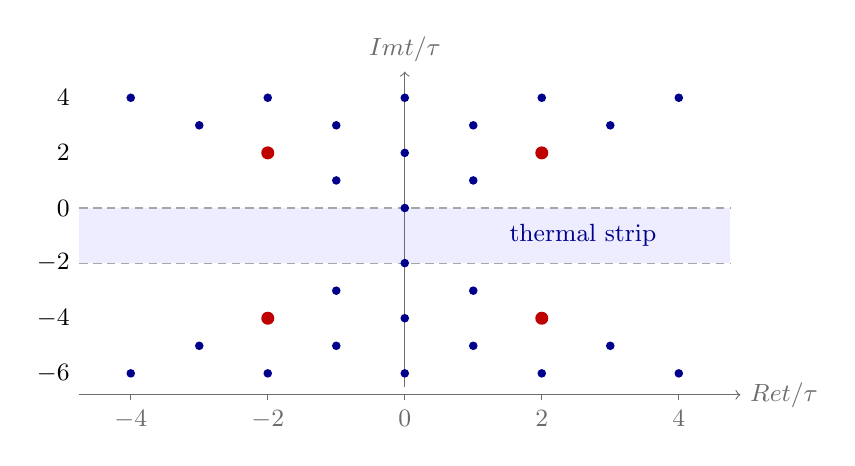
\begin{tikzpicture}[x=0.87cm,y=0.35cm, every node/.style={font=\small}]
 \fill[blue!7] (-4.75,-2) rectangle (4.75,0);
 \draw[gray!70,densely dashed] (-4.75,0) -- (4.75,0);
 \draw[gray!70,densely dashed] (-4.75,-2) -- (4.75,-2);
 \draw[->,gray!85!black] (0,-6.5) -- (0,4.95)
    node[above] {\(\operatorname{Im}t/\tau\)};
 \draw[->,gray!85!black] (-4.75,-6.78) -- (4.9,-6.78)
    node[right] {\(\operatorname{Re}t/\tau\)};
 \foreach \x in {-4,-2,0,2,4} {
   \draw[gray!85!black] (\x,-6.78) -- (\x,-6.98)
      node[below] {\(\x\)};
 }
 \foreach \y in {-6,-4,-2,0,2,4} {
   \node[left] at (-4.75,\y) {\(\y\)};
 }
 \node[blue!55!black] at (2.6,-1) {thermal strip};
 \foreach \n in {0,...,4} {
   \foreach \k in {0,...,\n} {
     \fill[blue!55!black] ({\n-2*\k},\n) circle[radius=1.55pt];
     \fill[blue!55!black] ({-\n+2*\k},{-\n-2}) circle[radius=1.55pt];
   }
 }
 \foreach \x in {-2,2} {
   \fill[red!75!black] (\x,2) circle[radius=2.35pt];
   \fill[red!75!black] (\x,-4) circle[radius=2.35pt];
 }
\end{tikzpicture}
\caption{Pole lattice of the Lovelock scalar Wightman function in units of
 \(\tau=\beta/2\). The red points are the two-bounce pair and its image
 under \(t\mapsto-t-\ii\beta\). The shaded open thermal strip contains
 no poles.}
\label{fig:poles}
\end{figure}
